\documentclass[11pt,a4paper]{article}

% ============ PACCHETTI ============
\usepackage[italian,provide=*]{babel}
\usepackage[utf8]{inputenc}
\usepackage[T1]{fontenc}
\usepackage[margin=2.5cm,headheight=14pt]{geometry}
\usepackage{booktabs}
\usepackage{array}
\usepackage{longtable}
\usepackage{graphicx}
\usepackage[dvipsnames]{xcolor}
\usepackage{enumitem}
\usepackage{amsmath}
\usepackage{fancyhdr}
\usepackage{titlesec}
\usepackage{tikz}
\usetikzlibrary{arrows.meta, positioning, fit, backgrounds}
\usepackage{tcolorbox}
\tcbuselibrary{skins,breakable}
\usepackage[hidelinks,colorlinks=true,linkcolor=RoyalBlue,urlcolor=RoyalBlue,citecolor=RoyalBlue]{hyperref}
\usepackage{parskip}
\usepackage{ragged2e}

% ============ COLORI ============
\definecolor{supsiblue}{HTML}{003366}
\definecolor{lightgray}{HTML}{F2F2F2}

% ============ INTESTAZIONI/PIÈ DI PAGINA ============
\pagestyle{fancy}
\fancyhf{}
\renewcommand{\headrulewidth}{0.4pt}
\fancyhead[L]{Esercizio System Management 0}
\fancyhead[R]{\thepage}
\fancyfoot[C]{SUPSI DTI -- Laboratorio System Management}

% ============ TITOLI SEZIONE ============
\titleformat{\section}{\normalfont\Large\bfseries\color{supsiblue}}{\thesection}{1em}{}
\titleformat{\subsection}{\normalfont\large\bfseries\color{supsiblue}}{\thesubsection}{1em}{}
\titleformat{\subsubsection}{\normalfont\normalsize\bfseries}{\thesubsubsection}{1em}{}

% ============ AMBIENTE NOTA ============
\newtcolorbox{nota}[1][]{
  colback=lightgray, colframe=supsiblue!60, boxrule=0.5pt,
  fonttitle=\bfseries, breakable, left=6pt, right=6pt, top=4pt, bottom=4pt,
  title={Nota}, #1
}

\newtcolorbox{placeholder}[1][]{
  colback=white, colframe=black!40, boxrule=0.6pt,
  breakable, left=6pt, right=6pt, top=6pt, bottom=6pt, #1
}

% ============ DATI DOCUMENTO ============
\title{\textbf{Esercizio System Management 0}\\[4pt]\Large Professional Servers and Virtualization Solutions}
\author{Gruppo 3: Andrea Pezzolla \& Giovanni Russo}
\date{SUPSI -- Dipartimento Tecnologie Innovative\\Corso: System Management -- A.A. 2026}

\begin{document}

\maketitle
\thispagestyle{empty}

\begin{center}
\textit{Riferimento: Esercizio System Management 0 -- A. Consoli, SUPSI DTI, Viganello 2026}
\end{center}

\vspace{1cm}

% ==================================================================
\section{Professional Servers}
% ==================================================================

\subsection{Punto 1 -- Il server fornito}

Il laboratorio si basa su due piattaforme hardware distinte, entrambe di classe enterprise: un sistema multi-nodo \textbf{Acer/Gateway GW2000h con nodi GW170hq F1} (rebranding Supermicro) e un sistema blade \textbf{HPE BladeSystem c7000} con nodi di calcolo \textbf{HPE ProLiant BL460c G7}. Di seguito la documentazione richiesta per entrambe le piattaforme.

\subsubsection{1a -- Scheda riassuntiva delle caratteristiche hardware}

\paragraph{Gateway (Acer) GW2000h w/GW170hq F1.}
Si tratta di un sistema \emph{multi-node} da 2U che ospita fino a quattro nodi server indipendenti nello stesso chassis, condividendo alimentazione e raffreddamento: una soluzione tipica per ambienti HPC e per data center che necessitano di alta densità di calcolo per unità di rack.

\begin{center}
\begin{longtable}{p{4.2cm}p{9.8cm}}
\toprule
\textbf{Caratteristica} & \textbf{Valore} \\
\midrule
\endfirsthead
\toprule
\textbf{Caratteristica} & \textbf{Valore} \\
\midrule
\endhead
Fattore di forma & Chassis 2U, fino a 4 nodi server indipendenti (\emph{multi-node}) \\
Nodi disponibili & GW170h F1 (Ethernet), GW170hd F1 (+ InfiniBand DDR), GW170hq F1 (+ InfiniBand QDR) \\
CPU per nodo & Fino a 2 $\times$ Intel Xeon serie 5500/5600 (Nehalem-EP / Westmere-EP), socket LGA1366 \\
RAM per nodo & 12 slot DDR3 registered/unbuffered ECC, tipicamente DDR3-1333 \\
Storage per nodo & Fino a 3 dischi SATA/SAS hot-swap da 3.5'' \\
Alimentazione & 2 $\times$ 1400 W ridondanti, certificazione 80 PLUS Gold \\
Raffreddamento & 4 ventole condivise dallo chassis \\
Rete & 2 porte Gigabit Ethernet integrate per nodo; modulo InfiniBand opzionale (DDR/QDR) sui modelli ``d''/``q'' \\
Management & Controller BMC integrato (iBMC), gestibile tramite \emph{Smart Console} web-based con KVM-over-IP \\
Target d'uso & Scale-out computing, cluster HPC di fascia media \\
\bottomrule
\end{longtable}
\end{center}

\paragraph{HPE ProLiant BL460c G7 (chassis HPE BladeSystem c7000).}
È un \emph{blade server} a due vie (\emph{2-way}) di settima generazione della linea ProLiant, alloggiato nell'enclosure c7000 che può ospitare fino a 16 blade a mezza altezza condividendo alimentazione, raffreddamento e connettività di rete/storage tramite moduli di interconnessione posteriori.

\begin{center}
\begin{longtable}{p{4.2cm}p{9.8cm}}
\toprule
\textbf{Caratteristica} & \textbf{Valore} \\
\midrule
\endfirsthead
\toprule
\textbf{Caratteristica} & \textbf{Valore} \\
\midrule
\endhead
Generazione & ProLiant G7 (settima generazione, piattaforma Intel Xeon serie 5600 ``Westmere-EP'') \\
CPU & Fino a 2 $\times$ Intel Xeon serie 5600 (es. X5670, X5675, E5649), socket LGA1366, chipset Intel 5520, 6 core/12 thread per CPU \\
RAM & 12 slot DIMM DDR3 registered ECC, 1333 MHz, fino a 384 GB (192 GB con moduli unbuffered) \\
Storage & 2 vani hot-swap SFF 2.5'' SAS/SATA, controller RAID Smart Array P410i \\
Rete integrata & 2 porte 10 Gigabit Ethernet (controller HP NC553i) verso i moduli Virtual Connect/Interconnect dello chassis \\
Video & Controller grafico integrato Matrox MGA G200 \\
Management & HPE Integrated Lights-Out 3 (iLO 3), supporto IPMI 2.0 e SMASH-CLP \\
Fattore di forma & Blade a mezza altezza, alloggiato in enclosure HPE BladeSystem c7000 (10U, fino a 16 blade) \\
\bottomrule
\end{longtable}
\end{center}

\subsubsection{1b -- L'interfaccia di management: scopo e funzionamento}

Tutti i server professionali moderni integrano, oltre alla normale scheda madre, un piccolo sistema di elaborazione indipendente chiamato \textbf{BMC (Baseboard Management Controller)}. Il BMC è un microcontrollore (spesso basato su architettura ARM, realizzato come system-on-chip) montato direttamente sulla scheda madre del server, dotato di proprio firmware, propria memoria e, di norma, di una propria porta Ethernet dedicata.

Il suo scopo è fornire funzionalità di \textbf{gestione out-of-band}, ossia indipendenti dallo stato del sistema operativo e persino dall'accensione del server stesso (finché è presente alimentazione ausiliaria). In pratica il BMC consente di:
\begin{itemize}[nosep]
    \item monitorare sensori hardware (temperature, velocità delle ventole, tensioni di alimentazione, stato degli alimentatori);
    \item accendere, spegnere o riavviare da remoto il server (power control);
    \item fornire una console remota KVM (tastiera/video/mouse) virtuale, incluso l'accesso alla fase di POST/BIOS;
    \item montare supporti virtuali (immagini ISO, chiavette USB virtuali) per installazioni da remoto;
    \item registrare log degli eventi hardware (SEL, System Event Log) e inviare allarmi (SNMP trap, e-mail);
    \item aggiornare firmware e BIOS da remoto;
    \item esporre un'interfaccia web e API (REST/Redfish o IPMI) per l'integrazione con strumenti di gestione centralizzata (es. HPE OneView, Dell OpenManage).
\end{itemize}

I vantaggi principali sono quindi la possibilità di amministrare un numero elevato di server da remoto, riducendo drasticamente la necessità di intervento fisico in sala macchine, e la possibilità di diagnosticare e risolvere problemi anche quando il sistema operativo non è raggiungibile o non è nemmeno installato.

\subsubsection{1c -- Differenza tra interfaccia di management e interfaccia di rete normale}

Sebbene entrambe possano condividere fisicamente la stessa porta RJ-45 (in modalità \emph{shared LOM}), si tratta di due piani completamente distinti:

\begin{center}
\begin{longtable}{p{4.8cm}p{4.6cm}p{4.6cm}}
\toprule
\textbf{Aspetto} & \textbf{Interfaccia di rete normale} & \textbf{Interfaccia di management} \\
\midrule
\endfirsthead
\toprule
\textbf{Aspetto} & \textbf{Interfaccia di rete normale} & \textbf{Interfaccia di management} \\
\midrule
\endhead
Chi la gestisce & Il sistema operativo (driver NIC) & Il BMC, indipendente dal S.O. \\
Disponibilità & Solo a server acceso e S.O. avviato & Sempre, finché c'è alimentazione ausiliaria (anche a server spento) \\
Traffico veicolato & Dati applicativi/utente & Dati di gestione (sensori, power control, KVM, firmware) \\
Stack di rete & Stack TCP/IP del sistema operativo & Stack di rete indipendente, gestito dal firmware del BMC \\
Protocolli tipici & HTTP(S), SMB, protocolli applicativi & IPMI, Redfish, SNMP, HTTPS verso la console web dedicata \\
Punto di guasto & Se il S.O. si blocca, l'interfaccia diventa irraggiungibile & Resta raggiungibile anche con S.O. bloccato o kernel panic \\
\bottomrule
\end{longtable}
\end{center}

In sintesi: l'interfaccia di rete ``normale'' è \emph{in-band} (dipende dal sistema operativo in esecuzione), mentre l'interfaccia di management è \emph{out-of-band} (opera a un livello sottostante, indipendente dal sistema operativo).

\subsubsection{1d -- Architettura hardware della motherboard e interfaccia di management}

A livello di scheda madre, il costruttore integra il BMC come componente separato dal percorso dati principale CPU--chipset--RAM, collegandolo tramite bus di servizio a bassa velocità (\emph{sideband}) piuttosto che tramite i bus ad alte prestazioni riservati al sistema operativo. I collegamenti tipici sono:

\begin{itemize}[nosep]
    \item \textbf{I2C/SMBus}: utilizzato dal BMC per interrogare sensori di temperatura, ventole e alimentatori, e per comunicare con i moduli di memoria (SPD) e altri componenti gestibili;
    \item \textbf{LPC o eSPI}: bus a bassa velocità storicamente usato per collegare il BMC al Super~I/O e condividere la console seriale/KVM con il chipset;
    \item \textbf{PCIe (dedicata al BMC)}: nei server più recenti il BMC dispone di un proprio collegamento PCIe per il traffico video e per l'accesso alle unità di storage tramite virtual media;
    \item \textbf{NC-SI (Network Controller Sideband Interface)}: un collegamento dedicato tra il BMC e la scheda di rete principale che consente al BMC di condividere una porta Ethernet fisica con il sistema operativo (\emph{shared LOM}), instradando il traffico di management su una VLAN o un canale logico separato;
    \item \textbf{Porta Ethernet dedicata}: in alternativa (o in aggiunta) il BMC può disporre di una propria porta di rete fisicamente separata (\emph{dedicated management port});
    \item \textbf{Memoria flash SPI dedicata}: il BMC esegue il proprio firmware da una memoria flash separata da quella del BIOS di sistema, per poter restare operativo anche se il firmware principale è corrotto.
\end{itemize}

Lo schema seguente riassume, in forma semplificata, questa architettura:

\begin{center}
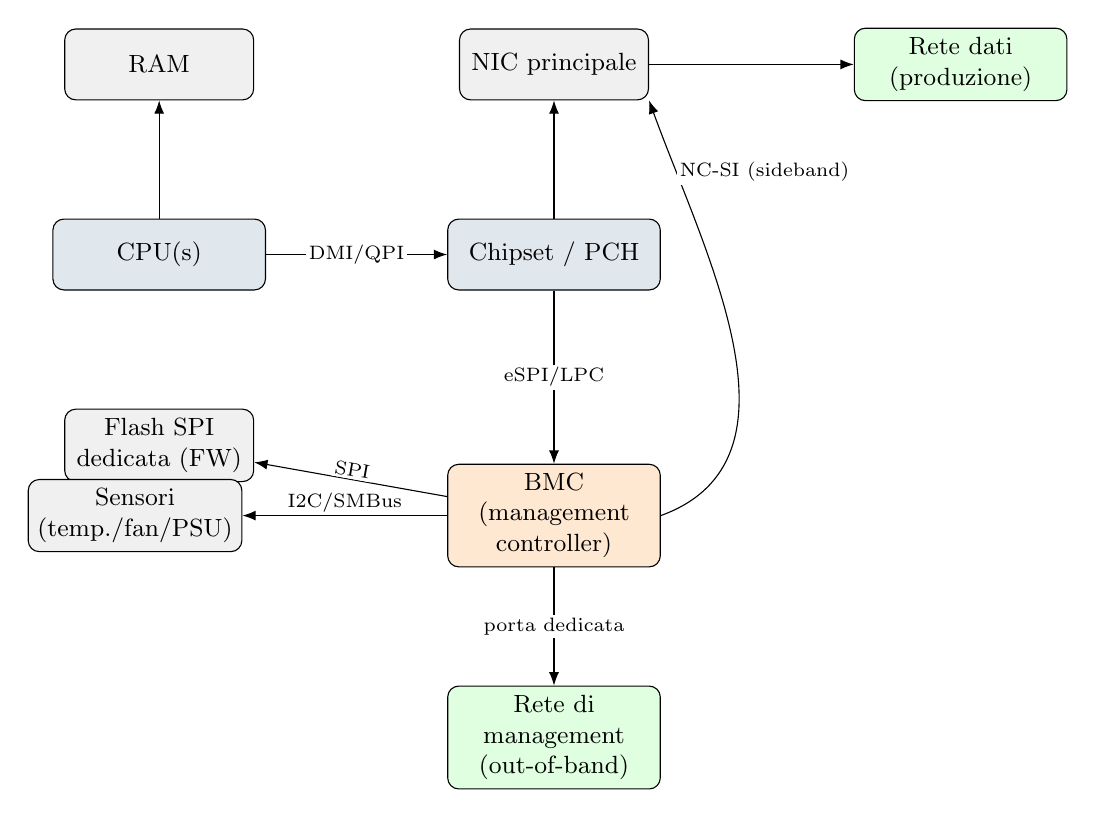
\begin{tikzpicture}[
    node distance=1.5cm and 2.6cm,
    box/.style={draw, rounded corners, minimum height=0.9cm, minimum width=2.7cm, align=center, font=\small},
    cpu/.style={box, fill=supsiblue!12},
    bmc/.style={box, fill=orange!18},
    ext/.style={box, fill=green!12},
    periph/.style={box, fill=gray!12, minimum width=2.4cm},
    lbl/.style={font=\scriptsize, align=center, fill=white, inner sep=1pt}
]
    % Riga superiore: percorso dati principale
    \node[periph] (ram) {RAM};
    \node[cpu, below=of ram] (cpu) {CPU(s)};
    \node[periph, right=of ram] (nic) {NIC principale};
    \node[cpu, below=of nic] (chipset) {Chipset / PCH};
    \node[ext, right=of nic] (lan) {Rete dati\\(produzione)};

    % Riga inferiore: BMC e periferia di management
    \node[bmc, below=2.2cm of chipset] (bmc) {BMC\\(management\\controller)};
    \node[periph, below=of cpu] (flash) {Flash SPI\\dedicata (FW)};
    \node[periph, left=of bmc] (sens) {Sensori\\(temp./fan/PSU)};
    \node[ext, below=of bmc] (mgmtnet) {Rete di\\management\\(out-of-band)};

    % Collegamenti percorso dati
    \draw[-Latex] (cpu) -- (ram);
    \draw[-Latex] (chipset) -- (nic);
    \draw[-Latex] (cpu) -- (chipset) node[lbl,midway]{DMI/QPI};
    \draw[-Latex] (nic) -- (lan);

    % Collegamenti management
    \draw[-Latex] (chipset) -- (bmc) node[lbl,midway,fill=white]{eSPI/LPC};
    \draw[-Latex] (bmc) -- (sens) node[lbl,midway,above]{I2C/SMBus};
    \draw[-Latex] (bmc) -- (flash) node[lbl,midway,above,sloped]{SPI};
    \draw[-Latex] (bmc) -- (mgmtnet) node[lbl,midway,fill=white]{porta dedicata};
    \draw[-Latex] (bmc.east) to[out=20,in=-70] node[lbl,pos=0.85,right]{NC-SI (sideband)} (nic.south east);
\end{tikzpicture}
\end{center}

Il BMC opera quindi come un ``computer nel computer'': possiede una propria CPU, una propria RAM, un proprio firmware e una propria connessione di rete, e resta attivo anche quando il server principale è spento, a patto che sia collegato all'alimentazione ausiliaria (standby power).

\subsection{Punto 2a -- Nomi commerciali dell'interfaccia di management per produttore}

Ogni produttore di server ha adottato un proprio marchio commerciale per la propria implementazione di BMC, pur basandosi tutti sullo standard aperto \textbf{IPMI (Intelligent Platform Management Interface)} e, più recentemente, sullo standard \textbf{Redfish} del DMTF.

\begin{center}
\begin{longtable}{p{3.5cm}p{10.5cm}}
\toprule
\textbf{Produttore} & \textbf{Nome dell'interfaccia di management} \\
\midrule
\endfirsthead
\toprule
\textbf{Produttore} & \textbf{Nome dell'interfaccia di management} \\
\midrule
\endhead
HPE & iLO -- Integrated Lights-Out (attualmente iLO~6) \\
DELL & iDRAC -- integrated Dell Remote Access Controller (attualmente iDRAC9) \\
LENOVO & XClarity Controller (XCC); nei modelli più datati IMM/IMM2 -- Integrated Management Module \\
IBM & IMM/IMM2 -- Integrated Management Module (linea System x, ora Lenovo) \\
SUPERMICRO & BMC con IPMI 2.0, gestito tramite le utility IPMIView / SuperDoctor / Supermicro Update Manager \\
Fujitsu & iRMC -- integrated Remote Management Controller \\
Oracle/Sun & ILOM -- Integrated Lights Out Manager \\
Cisco (UCS) & CIMC -- Cisco Integrated Management Controller \\
Acer/Gateway (rebrand Supermicro) & iBMC, gestito tramite \emph{Smart Console} \\
\bottomrule
\end{longtable}
\end{center}

\subsection{Punto 2b -- Memoria RAM per server}

\subsubsection{Differenze rispetto alla RAM dei normali computer utente}

La memoria RAM impiegata nei server professionali si differenzia da quella dei PC consumer per tre aspetti principali: \textbf{ECC}, \textbf{buffering/registrazione del segnale} e, in alcuni casi, \textbf{Chipkill}.

\begin{itemize}[nosep]
    \item \textbf{ECC (Error Correcting Code)}: ogni modulo dedica un chip aggiuntivo ogni 8 (quindi 9 chip invece di 8, o 18 invece di 16 per i moduli dual-rank) alla memorizzazione di bit di controllo calcolati con un codice di Hamming esteso (schema SECDED -- \emph{Single Error Correction, Double Error Detection}). Questo permette di correggere automaticamente un errore su un singolo bit e di rilevare (senza correggere) errori su due bit, evitando crash o corruzioni silenziose dei dati causate da eventi come i raggi cosmici o disturbi elettrici, particolarmente rilevanti quando si hanno centinaia di GB di RAM sempre attivi.
    \item \textbf{RDIMM (Registered DIMM)}: tra il controller di memoria della CPU e i chip DRAM viene inserito un piccolo componente chiamato \emph{register} (o RCD, Registering Clock Driver) che rigenera i segnali di indirizzo e comando. Questo riduce il carico elettrico sul controller di memoria, permettendo di installare molti più moduli per canale e quindi capacità complessive molto più elevate (centinaia di GB fino a diversi TB per socket) rispetto ai moduli UDIMM non bufferizzati tipici dei PC consumer.
    \item \textbf{LRDIMM (Load-Reduced DIMM)}: evoluzione dell'RDIMM che introduce anche buffer sui dati oltre che sugli indirizzi, per raggiungere le densità più elevate (moduli da centinaia di GB), tipicamente impiegata in server per virtualizzazione spinta o basi dati in-memory.
    \item \textbf{Chipkill (o tecnologie equivalenti come Advanced ECC/SDDC)}: sviluppata originariamente da IBM, distribuisce i bit di un singolo blocco di dati su chip DRAM diversi, in modo che il guasto completo di un intero chip di memoria (non solo un bit) venga comunque corretto, aumentando ulteriormente l'affidabilità rispetto al semplice ECC.
    \item \textbf{Memory mirroring / lockstep}: funzionalità disponibili su molte piattaforme server che replicano i dati su due canali di memoria distinti, così che il guasto di un intero canale o modulo non comprometta la continuità di servizio.
\end{itemize}

In sintesi, la maggiore affidabilità della RAM server deriva dalla combinazione di correzione automatica degli errori (ECC), dalla capacità di reggere configurazioni ad alta densità senza instabilità elettrica (moduli registered/load-reduced) e, nei sistemi più critici, dalla resilienza al guasto completo di un chip di memoria (Chipkill) o di un intero canale (mirroring).

\subsection{Punto 3 -- CPU server-grade}

Le CPU pensate per l'uso server (Intel Xeon, AMD EPYC) condividono spesso la stessa microarchitettura di base delle CPU consumer (Intel Core, AMD Ryzen), ma se ne differenziano per una serie di funzionalità orientate all'affidabilità, alla scalabilità e al funzionamento continuativo 24/7:

\begin{itemize}[nosep]
    \item \textbf{Supporto ECC}: le CPU server dispongono di un controller di memoria in grado di gestire moduli ECC (spesso anche registered/load-reduced), funzionalità tipicamente non abilitata o non certificata sulle CPU consumer di fascia mainstream;
    \item \textbf{Numero di canali di memoria e capacità massima}: da 6 a 12+ canali per socket contro i 2 (talvolta 4 su piattaforme HEDT) delle CPU desktop, con capacità massime che arrivano a diversi TB per socket contro poche decine/centinaia di GB;
    \item \textbf{Multi-socket}: supporto nativo a configurazioni a 2, 4 o 8 socket tramite interconnessioni dedicate (Intel UPI, AMD Infinity Fabric), impossibile sulle CPU consumer che restano single-socket;
    \item \textbf{Maggior numero di core/thread e cache L3}: orientati al throughput su carichi paralleli (virtualizzazione, database, calcolo scientifico) piuttosto che alle massime frequenze single-thread;
    \item \textbf{Maggior numero di linee PCIe}: fino a 128 lane per socket sulle piattaforme server più recenti, contro le 20--28 tipiche del desktop, necessarie per alimentare molteplici schede di rete, controller storage e acceleratori;
    \item \textbf{Funzionalità RAS (Reliability, Availability, Serviceability)}: tramite la Machine Check Architecture (MCA) le CPU server possono rilevare e, in molti casi, gestire in modo controllato errori hardware (es. errori di memoria, di cache, di bus) continuando l'esecuzione invece di bloccare immediatamente il sistema, funzionalità cruciale per servizi always-on;
    \item \textbf{Funzionalità di sicurezza e virtualizzazione avanzate}: estensioni per la virtualizzazione hardware (VT-x/VT-d, AMD-V), cifratura della memoria delle macchine virtuali (Intel TME/TDX, AMD SEV), spesso assenti o limitate sulle CPU consumer;
    \item \textbf{Certificazione e validazione}: le CPU server vengono validate per il funzionamento continuativo, con cicli di test più estesi e un firmware/microcode supportato per periodi molto più lunghi (anni) rispetto ai prodotti consumer;
    \item \textbf{Assenza di GPU integrata}: nella maggior parte dei casi non dispongono di un chip grafico integrato, poiché la gestione video è tipicamente demandata al BMC o a una scheda video dedicata di modeste prestazioni.
\end{itemize}

Il rovescio della medaglia è che le CPU server-grade hanno tipicamente frequenze di clock più contenute rispetto alle CPU consumer di pari fascia di prezzo, poiché l'obiettivo di design è il throughput aggregato su molti core piuttosto che le massime prestazioni single-thread.

\subsection{Punto 4 -- High Performance Computing: protocolli di rete}

\subsubsection{4a -- Protocolli per sistemi scientifici}

Nell'HPC scientifico (simulazioni numeriche, calcolo parallelo su cluster, meteorologia, genomica, fisica computazionale) l'obiettivo primario è minimizzare la latenza di comunicazione tra i nodi durante operazioni collettive (\emph{MPI all-reduce}, \emph{all-gather}), per cui si privilegiano tecnologie che offrono \textbf{RDMA (Remote Direct Memory Access)} nativo, ossia il trasferimento diretto tra le memorie dei nodi senza coinvolgere la CPU:

\begin{itemize}[nosep]
    \item \textbf{InfiniBand} (oggi controllato quasi in monopolio da NVIDIA/Mellanox): lo standard de-facto nei sistemi TOP500, con topologie a fat-tree o dragonfly e supporto nativo a RDMA, multicast e collective offload;
    \item \textbf{Intel/Cornelis Omni-Path}: alternativa proprietaria a InfiniBand, con un modello di offload parzialmente diverso (maggior carico sulla CPU rispetto a InfiniBand);
    \item \textbf{Cray Slingshot / Cray Aries}: interconnessioni proprietarie usate nei supercomputer Cray/HPE per sistemi exascale;
    \item \textbf{RoCE (RDMA over Converged Ethernet)}: porta i vantaggi RDMA su infrastrutture Ethernet standard, riducendo i costi rispetto a una fabric InfiniBand dedicata;
    \item \textbf{IP over InfiniBand (IPoIB)}: permette di veicolare traffico IP tradizionale sopra una fabric InfiniBand già presente, evitando reti Ethernet separate.
\end{itemize}

\subsubsection{4b -- Protocolli per soluzioni ICT finanziarie e industriali}

Nel settore finanziario (trading algoritmico/high-frequency trading, connettività verso le borse valori) la priorità è la \textbf{latenza deterministica dell'ordine di poche centinaia di nanosecondi} su reti Ethernet, poiché l'ecosistema (borse, provider di colocation, exchange) è quasi interamente basato su Ethernet piuttosto che su InfiniBand:

\begin{itemize}[nosep]
    \item \textbf{Ethernet a bassa latenza 10/25/40/100 GbE}: con switch \emph{cut-through} specializzati (es. serie Arista 7130/7150, Cisco Nexus 3548, Mellanox/NVIDIA Spectrum) che garantiscono latenze da poche centinaia di nanosecondi indipendentemente dalla dimensione del pacchetto;
    \item \textbf{RoCE / RDMA su Ethernet}: impiegato anche in ambito finanziario per la distribuzione di feed di mercato a bassissima latenza;
    \item \textbf{Protocolli applicativi FIX (Financial Information eXchange) e FAST}: standard de-facto per gli ordini e per la compressione dei feed di mercato ad alta frequenza, trasportati sopra le reti a bassa latenza citate sopra;
    \item \textbf{Fibre Channel (FC)}: ancora diffuso per le SAN storage in ambito bancario/finanziario dove è richiesta affidabilità e isolamento del traffico storage.
\end{itemize}

\subsubsection{Tabella riassuntiva dei throughput}

\begin{center}
\begin{longtable}{p{3.6cm}p{3.0cm}p{3.0cm}p{3.8cm}}
\toprule
\textbf{Tecnologia} & \textbf{Generazione} & \textbf{Throughput (link 4x, se applicabile)} & \textbf{Ambito tipico} \\
\midrule
\endfirsthead
\toprule
\textbf{Tecnologia} & \textbf{Generazione} & \textbf{Throughput (link 4x, se applicabile)} & \textbf{Ambito tipico} \\
\midrule
\endhead
InfiniBand & SDR (2003) & 8 Gb/s & HPC storico \\
InfiniBand & DDR (2006) & 16 Gb/s & HPC \\
InfiniBand & QDR (2008) & 32 Gb/s & HPC \\
InfiniBand & FDR (2011) & 54--56 Gb/s & HPC \\
InfiniBand & EDR (2014) & 100 Gb/s & HPC / AI \\
InfiniBand & HDR (2018) & 200 Gb/s & HPC / AI \\
InfiniBand & NDR (2021) & 400 Gb/s & HPC / AI \\
Ethernet & 10 GbE & 10 Gb/s & Enterprise / financial \\
Ethernet & 25/40 GbE & 25--40 Gb/s & Enterprise / financial \\
Ethernet & 100 GbE & 100 Gb/s & Data center / financial \\
Fibre Channel & FC8 / FC16 & 8 / 16 Gb/s & SAN storage \\
\bottomrule
\end{longtable}
\end{center}

\subsection{Punto 5 -- Il termine ``Blade''}

Con \textbf{server blade} si indica un server progettato come modulo compatto (la ``lama'', in inglese \emph{blade}) privo di alimentatori, ventole e talvolta anche di alcune interfacce di rete proprie, che viene inserito in uno \textbf{chassis/enclosure} condiviso insieme ad altri blade dello stesso tipo. Lo chassis fornisce centralmente alimentazione ridondante, raffreddamento, connettività di rete/storage (tramite moduli di interconnessione posteriori) e un unico punto di gestione per tutti i blade alloggiati. Il vantaggio principale è la massima densità di calcolo per unità di spazio rack e la semplificazione del cablaggio e della gestione rispetto a un pari numero di server rack tradizionali (\emph{rack-mount}).

Esempi di sistemi blade di produttori differenti:

\begin{itemize}[nosep]
    \item \textbf{HPE BladeSystem c7000}: enclosure da 10U che ospita fino a 16 blade a mezza altezza (es. HPE ProLiant BL460c), con moduli Virtual Connect per la connettività di rete/SAN;
    \item \textbf{Dell PowerEdge M1000e}: enclosure da 10U per blade PowerEdge M-series, con gestione centralizzata tramite pannello LCD frontale;
    \item \textbf{IBM BladeCenter} (ora Lenovo Flex System): una delle prime piattaforme blade enterprise di larga diffusione, nota per la robustezza dell'architettura;
    \item \textbf{Cisco UCS 5108}: chassis da 6U che integra fino a 8 blade B-series, distintivo per l'integrazione nativa tra networking e gestione dei server tramite Cisco UCS Manager;
    \item \textbf{Acer/Gateway GW2000h}: sistema multi-node 2U analizzato al punto 1, concettualmente affine ai blade pur essendo di dimensioni più contenute.
\end{itemize}

\subsection{Punto 6 -- Il termine ``Unit'' / ``HE''}

Con \textbf{Unit} (abbreviato \textbf{U}, in tedesco \textbf{HE}, \emph{H\"oheneinheit}) si indica l'unità di misura standard dell'altezza delle apparecchiature destinate a un armadio rack a 19 pollici, definita dallo standard \textbf{EIA-310}. Una unità corrisponde a \textbf{1.75 pollici}, pari a \textbf{44.45 mm}. Un dispositivo di altezza doppia si definisce ``2U'' (3.5 pollici / 88.9 mm), uno triplo ``3U'' (5.25 pollici / 133.35 mm) e così via.

\subsection{Punto 7 -- Quante Unit può contare un armadio rack}

Un armadio rack a 19 pollici a \textbf{piena altezza} conta tipicamente \textbf{42U} (circa 1.87 m di spazio utile), sebbene esistano varianti comuni da \textbf{45U, 47U e 48U} per ambienti ad alta densità, e rack a ``mezza altezza'' da \textbf{18--22U} (circa 0.9 m) per installazioni più compatte o da ufficio.

\newpage
% ==================================================================
\section{Virtualization Solutions}
% ==================================================================

\subsection{Punto 8 -- Sistemi di virtualizzazione: diffusione sul mercato}

\begin{center}
\begin{longtable}{p{3.2cm}p{2.6cm}p{7.6cm}}
\toprule
\textbf{Sistema} & \textbf{Anno di creazione} & \textbf{Note sulla diffusione} \\
\midrule
\endfirsthead
\toprule
\textbf{Sistema} & \textbf{Anno di creazione} & \textbf{Note sulla diffusione} \\
\midrule
\endhead
VMware (ESX/ESXi) & 1998 (fondazione VMware); primo prodotto VMware Workstation nel 1999, ESX Server nel 2001 & Storicamente il hypervisor dominante in ambito enterprise (indagini di settore degli anni 2010 lo indicavano oltre l'80\% delle installazioni server-side). Dopo l'acquisizione da parte di Broadcom (2023) e i cambiamenti di licensing, nel 2025--2026 si osserva una migrazione crescente verso alternative (KVM/Proxmox, Hyper-V, Nutanix AHV) \\
Xen & 2003 (primo rilascio stabile, Università di Cambridge) & Molto diffuso storicamente nel cloud pubblico (AWS lo ha utilizzato per anni come base di EC2) e tramite Citrix XenServer; base anche di Oracle VM. Progressivamente eroso da KVM \\
QEMU & 2003 & Emulatore/virtualizzatore multipiattaforma (x86, ARM, PowerPC, \dots); da solo offre virtualizzazione software, ma è anche il motore utilizzato da KVM per l'emulazione dei dispositivi virtuali \\
KVM & 2006/2007 (annunciato ottobre 2006, incluso nel kernel Linux 2.6.20, febbraio 2007) & Diventato lo standard \emph{open source} di riferimento nel cloud (OpenStack, Proxmox VE, Red Hat/oVirt) e adottato internamente da grandi cloud provider (AWS Nitro, Google Cloud, Alibaba Cloud); in forte crescita relativa dal 2023--2026 anche in ambito enterprise on-premise \\
\bottomrule
\end{longtable}
\end{center}

\subsection{Punto 9 -- Versioni di VMware ESXi}

\subsubsection{Versione più recente}

Alla data di redazione di questo documento (settembre 2026), la versione più recente e commercialmente disponibile della piattaforma è \textbf{VMware vSphere / ESXi 9.1}, rilasciata da Broadcom il \textbf{12 maggio 2026} (con successivi aggiornamenti puntuali, l'ultimo dei quali -- 9.1.0.0200 -- datato 13 luglio 2026). La release principale precedente, \textbf{ESXi 9.0}, era stata rilasciata il 17 giugno 2025.

\subsubsection{Storico delle versioni principali}

\begin{center}
\begin{longtable}{p{2.6cm}p{3.2cm}p{7.8cm}}
\toprule
\textbf{Versione} & \textbf{Data di rilascio} & \textbf{Note} \\
\midrule
\endfirsthead
\toprule
\textbf{Versione} & \textbf{Data di rilascio} & \textbf{Note} \\
\midrule
\endhead
ESX Server 1.0 & 2001 & Primo hypervisor bare-metal di VMware \\
ESX 2.x / 3.x & 2003 / 2006 & Introduzione di VMFS, prime funzionalità di clustering \\
ESXi 3.5 & 2007--2008 & Prima variante ``ESXi'' senza Service Console basata su Linux \\
ESXi 4.x & 2009 & Introduzione vSphere come suite completa \\
ESXi 5.0 / 5.1 / 5.5 & 2011 / 2012 / 2013 & Consolidamento della piattaforma, vSAN introdotto in 5.5 \\
ESXi 6.0 & Marzo 2015 & Supporto a configurazioni cluster più ampie \\
ESXi 6.5 & Novembre 2016 & Introduzione del vSphere Client HTML5 \\
ESXi 6.7 & Aprile 2018 & Ultima versione con Service Console EOL nel 2022 \\
ESXi 7.0 & Aprile 2020 & Nuovo layout di partizionamento, limite di 32 core per licenza per CPU \\
ESXi 8.0 & Ottobre 2022 & Supporto DPU (Data Processing Unit), miglioramenti device passthrough \\
ESXi 9.0 & Giugno 2025 & Prima release principale interamente sotto il marchio Broadcom \\
ESXi 9.1 & Maggio 2026 & Versione più recente al momento della stesura di questo documento \\
\bottomrule
\end{longtable}
\end{center}

\subsubsection{Requisiti hardware richiesti dalle versioni 6.7, 7.0 e 8.0}

\begin{center}
\begin{longtable}{p{2.4cm}p{3.6cm}p{3.0cm}p{4.6cm}}
\toprule
\textbf{Versione} & \textbf{CPU minima} & \textbf{RAM minima} & \textbf{Note aggiuntive} \\
\midrule
\endfirsthead
\toprule
\textbf{Versione} & \textbf{CPU minima} & \textbf{RAM minima} & \textbf{Note aggiuntive} \\
\midrule
\endhead
ESXi 6.7 & CPU x86-64 con almeno 2 core, bit NX/XD abilitato nel BIOS & 4 GB fisici (8 GB consigliati per ambienti di produzione) & Supporto boot UEFI; boot device minimo 1 GB \\
ESXi 7.0 & CPU x86-64 con almeno 2 core, bit NX/XD abilitato nel BIOS & 4 GB fisici (8 GB consigliati) & Boot device minimo 8 GB (USB/SD) o 32 GB (altri dispositivi); nuovo layout di partizionamento non retrocompatibile con il ripristino verso 6.7 \\
ESXi 8.0 & CPU x86-64 con almeno 2 core, bit NX/XD abilitato nel BIOS & 8 GB fisici (12 GB consigliati) & Requisito di RAM minima raddoppiato rispetto alla 7.0; introdotto supporto nativo alle DPU \\
\bottomrule
\end{longtable}
\end{center}

In tutti i casi è inoltre richiesto il supporto hardware alla virtualizzazione (Intel VT-x o AMD-V) per l'esecuzione di macchine virtuali a 64 bit e almeno una scheda di rete Gigabit Ethernet o superiore; la compatibilità hardware va sempre verificata sulla VMware/Broadcom Compatibility Guide (HCL), poiché il supporto ai singoli modelli di server/CPU/adattatori varia da versione a versione.

\subsection{Punto 10 -- Il termine ``VMotion''}

\textbf{vMotion} (in origine ``VMotion'') è la tecnologia di \textbf{live migration} di VMware che consente di spostare una macchina virtuale in esecuzione da un host ESXi a un altro \textbf{senza interruzione di servizio}, senza perdita di connettività di rete e senza downtime percepibile dagli utenti/applicazioni.

Il meccanismo, in estrema sintesi, prevede:
\begin{enumerate}[nosep]
    \item un controllo preliminare di compatibilità tra host di origine e di destinazione (CPU compatibili o \emph{Enhanced vMotion Compatibility} attiva a livello di cluster);
    \item la copia iterativa della memoria RAM della VM dall'host sorgente all'host di destinazione, mentre la VM continua a girare sull'host sorgente (\emph{pre-copy}): ad ogni iterazione vengono ritrasmesse solo le pagine di memoria modificate nel frattempo (\emph{dirty pages});
    \item quando la quantità di memoria ``sporca'' residua è sufficientemente piccola, la VM viene brevemente sospesa (uno \emph{stun} dell'ordine dei millisecondi), lo stato residuo di CPU/memoria/registri viene trasferito e la VM riprende l'esecuzione sull'host di destinazione;
    \item il traffico di rete verso la VM viene reindirizzato in modo trasparente (la VM mantiene lo stesso indirizzo MAC e la stessa identità di rete).
\end{enumerate}

Requisiti tipici: storage condiviso tra gli host (SAN/NAS) -- oppure, con \emph{Storage vMotion}, anche i file disco possono essere spostati contestualmente -- e una rete dedicata a banda sufficiente (Gigabit Ethernet o superiore) per il traffico di vMotion.

vMotion è alla base di funzionalità di livello superiore come \textbf{DRS} (\emph{Distributed Resource Scheduler}, bilanciamento automatico del carico tra gli host di un cluster) e consente di eseguire manutenzione hardware pianificata su un host senza dover fermare i servizi in esso ospitati.

\subsection{Punto 11 -- Videate del sistema di gestione VMware}

Questo punto richiede la raccolta di schermate dal proprio ambiente VMware di laboratorio (host ESXi/vCenter assegnato al gruppo). Di seguito l'elenco delle videate richieste dal testo dell'esercizio, da acquisire direttamente dal vSphere Client (HTML5) o dall'interfaccia host locale, con una breve indicazione di dove reperirle:

\begin{center}
\begin{longtable}{p{6.2cm}p{6.6cm}}
\toprule
\textbf{Videata richiesta} & \textbf{Dove acquisirla nel vSphere Client} \\
\midrule
\endfirsthead
\toprule
\textbf{Videata richiesta} & \textbf{Dove acquisirla nel vSphere Client} \\
\midrule
\endhead
Lista delle macchine virtuali & Host/vCenter $\rightarrow$ scheda \emph{VMs} (o \emph{Virtual Machines} nel menu Navigator) \\
Lista dei dischi del datastore & Host $\rightarrow$ \emph{Storage} $\rightarrow$ scheda \emph{Devices} \\
Lista dei virtual switch & Host $\rightarrow$ \emph{Networking} $\rightarrow$ scheda \emph{Virtual switches} \\
Dettagli di una macchina virtuale & Selezionare la VM $\rightarrow$ scheda \emph{Summary}/\emph{Monitor} \\
Dettagli di un virtual switch & \emph{Networking} $\rightarrow$ selezionare lo switch $\rightarrow$ topologia e porte associate \\
Dettagli di un disco del datastore & \emph{Storage} $\rightarrow$ selezionare il datastore $\rightarrow$ scheda \emph{Configure}/\emph{Files} \\
Utilizzo risorse di una VM & Selezionare la VM $\rightarrow$ scheda \emph{Monitor} $\rightarrow$ \emph{Performance} (CPU/Memoria/Disco/Rete) \\
Utilizzo totale delle risorse dell'host & Host $\rightarrow$ scheda \emph{Summary} (pannelli CPU/Memoria/Storage in alto, come visibile anche nell'esempio di schermata riportato nel testo dell'esercizio) \\
Impostazione dell'indirizzo IPv4 dell'host & Host $\rightarrow$ \emph{Manage}/\emph{Networking} $\rightarrow$ \emph{VMkernel NICs} $\rightarrow$ modifica delle impostazioni IPv4 \\
\bottomrule
\end{longtable}
\end{center}

\begin{placeholder}
\centering
\vspace{2cm}
\textit{[Inserire qui lo screenshot: ``Lista delle macchine virtuali''] }
\vspace{2cm}
\end{placeholder}

\begin{placeholder}
\centering
\vspace{2cm}
\textit{[Inserire qui lo screenshot: ``Lista dei dischi del datastore'']}
\vspace{2cm}
\end{placeholder}

\begin{placeholder}
\centering
\vspace{2cm}
\textit{[Inserire qui lo screenshot: ``Lista dei virtual switch'']}
\vspace{2cm}
\end{placeholder}

\begin{placeholder}
\centering
\vspace{2cm}
\textit{[Inserire qui lo screenshot: ``Dettagli di una macchina virtuale'']}
\vspace{2cm}
\end{placeholder}

\begin{placeholder}
\centering
\vspace{2cm}
\textit{[Inserire qui lo screenshot: ``Dettagli di un virtual switch'']}
\vspace{2cm}
\end{placeholder}

\begin{placeholder}
\centering
\vspace{2cm}
\textit{[Inserire qui lo screenshot: ``Dettagli di un disco del datastore'']}
\vspace{2cm}
\end{placeholder}

\begin{placeholder}
\centering
\vspace{2cm}
\textit{[Inserire qui lo screenshot: ``Utilizzo risorse di una VM'']}
\vspace{2cm}
\end{placeholder}

\begin{placeholder}
\centering
\vspace{2cm}
\textit{[Inserire qui lo screenshot: ``Utilizzo totale delle risorse dell'host'']}
\vspace{2cm}
\end{placeholder}

\begin{placeholder}
\centering
\vspace{2cm}
\textit{[Inserire qui lo screenshot: ``Impostazione IPv4 dell'host'']}
\vspace{2cm}
\end{placeholder}

\subsection{Punto 12 -- La funzionalità ``Maintenance Mode''}

La \textbf{Maintenance Mode} (modalità manutenzione) è uno stato in cui può essere posto un host ESXi appartenente a un cluster, tipicamente prima di interventi che richiedono l'arresto o il riavvio dell'host stesso (aggiornamento firmware/BIOS, aggiornamento della versione ESXi, sostituzione di componenti hardware, manutenzione fisica).

Quando un host entra in maintenance mode:
\begin{itemize}[nosep]
    \item non è più possibile accendere nuove macchine virtuali su quell'host, né effettuare vMotion \emph{verso} di esso;
    \item se il cluster dispone di \textbf{DRS} attivo, le macchine virtuali in esecuzione vengono automaticamente migrate (via vMotion) verso altri host del cluster, senza interruzione di servizio;
    \item una volta che tutte le VM sono state spostate (o spente, se non è possibile la migrazione a caldo), l'host risulta pronto per l'intervento di manutenzione;
    \item al termine dell'intervento, l'host viene fatto uscire dalla maintenance mode e torna disponibile per l'assegnazione di nuovi carichi di lavoro.
\end{itemize}

Si utilizza quindi ogni volta che è necessario intervenire su un host fisico senza impattare la disponibilità dei servizi ospitati: è uno degli scopi pratici principali per cui la tecnologia vMotion (punto 10) è stata introdotta.

\subsection{Punto 13 -- Documentare lo stato di un host VMware ed esportarne le informazioni}

VMware/Broadcom mette a disposizione diversi strumenti, nativi e di terze parti, per produrre una documentazione completa dello stato di un host (risorse, VM, datastore, networking):

\begin{itemize}[nosep]
    \item \textbf{vSphere Client -- esportazione singola VM/host}: dal client HTML5 è possibile esportare direttamente informazioni di riepilogo di host e macchine virtuali (es. \emph{Export System Logs}) senza strumenti esterni;
    \item \textbf{\texttt{vm-support}}: script incluso in ogni host ESXi che raccoglie in un unico archivio compresso log di sistema, configurazione, informazioni hardware e stato delle VM -- lo strumento standard per la raccolta rapida di un ``bundle'' diagnostico completo, anche da riga di comando (SSH) o dall'interfaccia web (\emph{Export System Logs});
    \item \textbf{\texttt{esxcli} / \texttt{esxtop}}: comandi da riga di comando eseguibili via SSH sull'host, per interrogare puntualmente storage, networking, hardware e prestazioni ed esportarne l'output in file di testo;
    \item \textbf{PowerCLI}: modulo PowerShell ufficiale VMware che consente di interrogare in modo scriptabile host e vCenter (VM, datastore, reti, configurazione hardware) ed esportare i risultati in CSV/HTML per la reportistica;
    \item \textbf{RVTools}: strumento gratuito di terze parti molto diffuso, che si collega a vCenter/host ESXi ed esporta in un'unica cartella Excel decine di tabelle (VM, host, datastore, reti, snapshot, licenze) pronte per essere allegate a un rapporto;
    \item \textbf{VMware Aria Operations (ex vRealize Operations)}: soluzione enterprise di monitoraggio e reportistica che fornisce dashboard e report periodici automatizzati sull'utilizzo delle risorse a livello di infrastruttura;
    \item \textbf{API REST / Redfish e vSphere API}: per un'integrazione completamente automatizzata con strumenti di documentazione o CMDB aziendali, interrogabili anche senza l'interfaccia grafica.
\end{itemize}

Per un rapporto di laboratorio come il presente, la combinazione più semplice ed efficace è tipicamente: schermate manuali dal vSphere Client per la parte illustrativa (punto 11), affiancate da un export \texttt{vm-support} o da un report RVTools per la documentazione tecnica di dettaglio.

\end{document}